\chapter{SYSTEM DESIGN}
\label{ch:systemdesign}

This chapter records the requirements the system was built against, the feasibility assessment made before construction, and the design of the delivered system. The diagrams describe what was built and not what was proposed; the block diagram in particular differs from the one in the proposal, for the reasons given in Section~\ref{sec:deploychange}.

\section{Requirement Specification}

The requirements are separated by what each one constrains. The software and hardware subsections record what the system depends on, and they distinguish the offline stages, which ran on the team's own laptops, from what a user's device has to supply at the moment of use. The functional subsection states what the system does. The non-functional subsection states the properties it has to hold while doing it. Two of those properties shaped the design more than any functional entry did: silence in place of a wrong answer, and preprocessing that is identical in training and in deployment. Each requirement is phrased so that it names something checkable against the evidence in Chapter~\ref{ch:results} rather than an intention.

\subsection{Software Requirements}

\begingroup
\small
\begin{longtable}{|p{3.4cm}|p{9.6cm}|}
        \caption{Software used, and the role of each component}
        \label{tab:software} \\
        \hline
        \textbf{Component} & \textbf{Role in the system} \\
        \hline
        \endfirsthead
        \multicolumn{2}{l}{\itshape Table \thetable\ (continued from previous page)} \\
        \hline
        \textbf{Component} & \textbf{Role in the system} \\
        \hline
        \endhead
        \hline
        \multicolumn{2}{r}{\itshape continued on next page} \\
        \endfoot
        \hline
        \endlastfoot
        Python 3.11 & Recording, preprocessing, training, and the fallback server. The version is pinned because MediaPipe and TensorFlow resolve to a compatible set only on 3.11. \\
        \hline
        MediaPipe Holistic & Pretrained pose and hand tracking. Produces the 225-value feature vector for each frame, offline during recording and again on the fallback server at inference. \\
        \hline
        MediaPipe Pose and Hand Landmarker & The mobile-supported successors to Holistic. Produce the same 225 values on the phone, since Holistic has no mobile build. \\
        \hline
        OpenCV & Camera capture, frame decoding, colour conversion, and the horizontal mirror applied before detection. \\
        \hline
        TensorFlow / Keras & Building and training the BiLSTM, and exporting it. \\
        \hline
        NumPy & Landmark arrays, normalisation arithmetic, and the compiled dataset tensors. \\
        \hline
        scikit-learn & Stratified splits, class weights, and the confusion matrix and classification report. \\
        \hline
        Matplotlib & Training curves, the confusion matrix, and the frame-count histogram. \\
        \hline
        TensorFlow Lite & The deployed model format. Runs on the phone, and on the fallback server through a runtime that does not require full TensorFlow. \\
        \hline
        FastAPI and Uvicorn & The fallback server and its WebSocket endpoint. \\
        \hline
        Docker & Packaging the server with its model and runtime so deployment does not depend on the host environment. \\
        \hline
        Flutter and Dart & The Android client: camera capture, frame conversion, the ported preprocessing, the WebSocket protocol for the fallback path, and playback of the recorded Nepali phrase through \texttt{just\_audio}. \\
        \hline
        FFmpeg & Preparing the Nepali voice recordings: silence trimming, loudness normalisation, and conversion to the single audio format every playback target accepts. Used offline by a build script, not at run time. \\
        \hline
        Kotlin & The Android bridge that runs the two landmark models and assembles the 225-value vector on the device. \\
        \hline
        Git and GitHub & Version control for the code, and the mechanism by which eight signers' recordings were merged into one dataset. \\
\end{longtable}
\endgroup

\subsection{Hardware Requirements}

Training and evaluation ran on an ordinary laptop with no GPU. The model has 192{,}007 parameters and each evaluation fold completes in minutes on a processor alone, so no accelerator was required at any stage. Data collection needed only a webcam. At use time the system needs an Android phone with a camera and roughly 18 megabytes of storage for the bundled models, and nothing else. There is no network connection, no server, and no accelerator, since the landmarkers fall back to the processor when no GPU delegate is available. The fallback server path additionally needs a machine to run the container and a network the phone can reach.

\subsection{Functional Requirements}

\begin{enumerate}
    \item \textbf{Dataset recording.} The system shall record clips of each target phrase, extract the 225-value feature vector for each frame, and store each clip with its class, signer identity, frame count, and per-block detection rates.
    \item \textbf{Preprocessing.} The system shall normalise every clip against the shoulder-midpoint and wrist anchors and standardise it to the fixed sequence length, by a definition held in one place, with any reimplementation of it verified against that definition rather than trusted.
    \item \textbf{Phrase recognition.} Given a captured sequence, the system shall produce a probability distribution over the seven classes.
    \item \textbf{On-device operation.} The system shall perform landmark extraction and classification on the user's phone, so that recognition does not depend on a network connection at the moment of use.
    \item \textbf{Rejection of unknown input.} The system shall be trained with an explicit negative class covering non-signing motion. An input unlike any of the six target phrases then has a class to be assigned to, instead of being forced into one of them. The system shall report such an input as unrecognised rather than announcing it.
    \item \textbf{Confidence thresholding.} The system shall emit a phrase only when confidence reaches the configured threshold, and shall remain silent otherwise.
    \item \textbf{Text and speech output.} On an accepted recognition the system shall display the phrase on screen in English and Nepali and play the recorded Nepali phrase aloud. The audio shall be bundled with the application, so that output does not depend on a voice being installed on the device.
    \item \textbf{Live capture.} The client shall process frames while the user signs and present the result when signing ends, without the user needing to time or trim the recording.
    \item \textbf{Evaluation reporting.} The system shall report signer-independent accuracy, a pooled confusion matrix, and per-class precision, recall, and F1.
\end{enumerate}

\subsection{Non-Functional Requirements}

\begin{enumerate}
    \item \textbf{Response time.} A result shall be returned promptly enough that the interaction feels immediate, which requires overlapping landmark extraction with signing instead of performing it after capture.
    \item \textbf{Silence over error.} A wrong announcement is more harmful than no announcement. The system shall prefer refusing to answer.
    \item \textbf{Train and serve equivalence.} The features presented to the model at inference shall be produced by the same procedure that produced the training features. Where the deployment platform makes sharing the code impossible, the reimplementation shall be pinned to the original by generated fixtures that fail on divergence.
    \item \textbf{Cost.} The system shall use only free and open-source components and shall require no GPU or paid service.
    \item \textbf{Privacy.} No video of any signer shall be stored, and no image shall leave the user's phone during recognition. The dataset holds landmark coordinates only.
    \item \textbf{Usability under stress.} The interface shall need one action to start and one to finish, with large readable output, and shall require no configuration before a first recognition.
    \item \textbf{Diagnosability.} The client shall display what the recogniser observed per frame, so that a failure during use can be attributed instead of guessed at, and shall retain the landmark clip behind each attempt for later inspection.
    \item \textbf{Maintainability.} The feature layout, normalisation anchors, sequence length, and thresholds shall be defined in one place and imported everywhere else.
\end{enumerate}

\section{Feasibility Assessment}

\subsection{Economic Feasibility}
Every component is free and open-source. Development used laptops the team already owned, and no GPU, paid dataset, or cloud service was purchased at any point. Because recognition runs on the phone, the delivered system has no recurring cost at all: there is no server to keep running and no traffic to pay for. The optional fallback server, if deployed, is the only component that would carry one.

\subsection{Technical Feasibility}
The enabling technologies are mature. MediaPipe provides pretrained tracking that needs no training data of its own, on the desktop and on the phone alike, and the BiLSTM is a well-understood architecture for sequence classification. Reducing each frame to 225 values lowers the dimensionality enough that a few hundred clips suffice, which is what made a custom dataset viable within the project timeline, and it leaves a classifier small enough to run on a phone. The principal risk was never the model; it was whether an authentic dataset could be collected at all, which depended on access to the Deaf community.

\subsection{Operational Feasibility}
The interaction is two taps: one to begin signing and one to end. The system needs no specialised hardware on the user's side beyond a phone, no network at the moment of use, no account, and no configuration before the first recognition. It addresses a need the Deaf organisations consulted during this project confirmed is real, and can be demonstrated live. The main operational weakness is now the speed of landmark extraction on modest hardware, which is what the temporal correction of Section~\ref{sec:ondevice} exists to absorb and what the fallback server exists to escape.

\section{Use Case Diagram}

Figure~\ref{fig:usecase} shows the actors and their interactions. The Deaf Signer starts a session and performs an emergency phrase. The Hearing Person is the recipient of the output, reading the displayed phrase and hearing it spoken; they do not operate the system. The Developer role covers the offline work: recording and labelling the dataset, training and evaluating the model, and packaging the trained model into the application.

\begin{figure}[htbp]
    \centering
    % trim removes the uneven blank border baked into the exported PNG, which
    % otherwise makes the drawing sit left of centre
    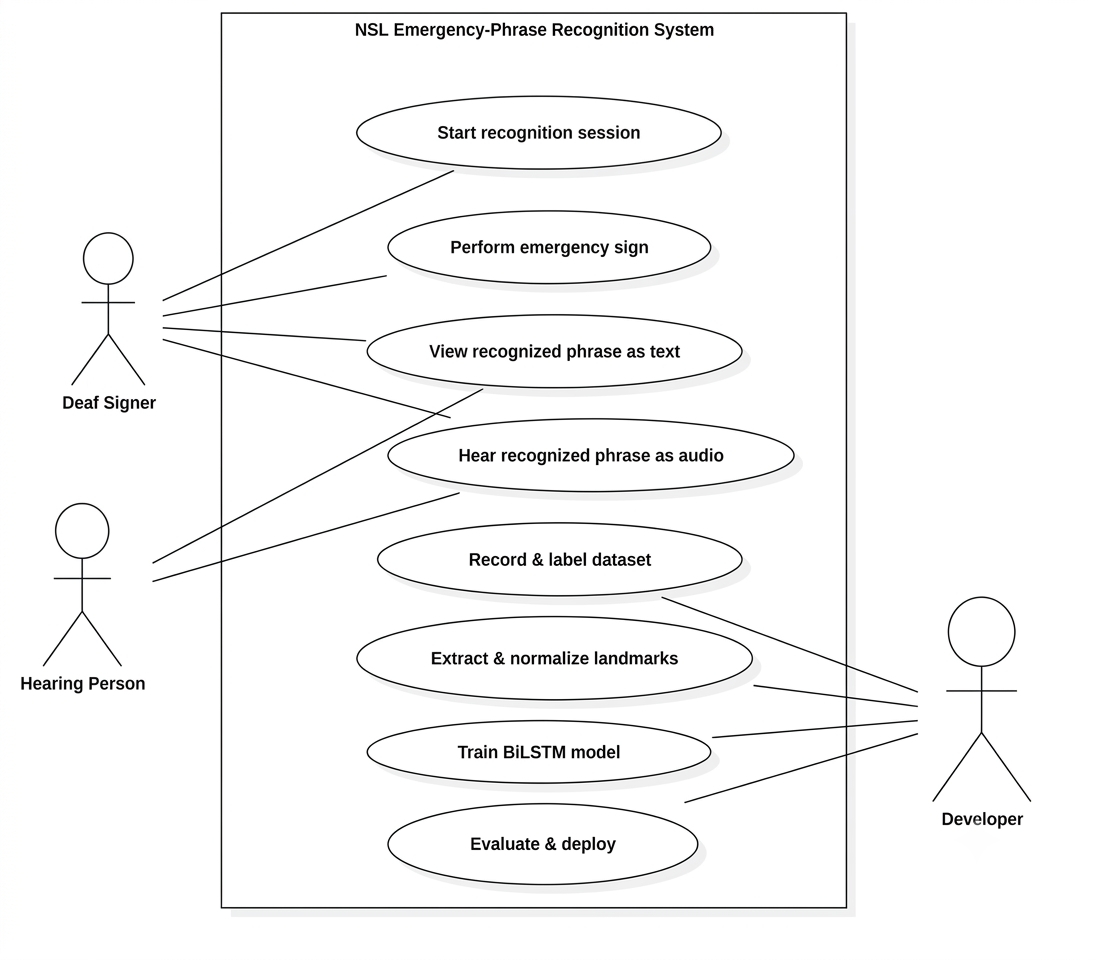
\includegraphics[width=0.70\textwidth, trim=21 43 66 12, clip]{img/usecase.png}
    \caption{Use case diagram}
    \label{fig:usecase}
\end{figure}

\section{System Block Diagram}

The system has three parts. An offline path builds the model, the phone reproduces the offline preprocessing at inference time and runs the classifier, and a server offers the same path over a network for devices that cannot. Figure~\ref{fig:blockdiagram} shows all three and the preprocessing definition that connects them.

\begin{figure}[htbp]
    \centering
    \resizebox{\textwidth}{!}{%
    \begin{tikzpicture}[
        box/.style={rectangle, rounded corners=2pt, fill=dfill, draw=dline,
                    text width=2.3cm, align=center, font=\sffamily\scriptsize,
                    minimum height=1.15cm, inner sep=3pt},
        store/.style={box, fill=white, draw=dgrey, dashed},
        shared/.style={box, fill=dfilla, draw=dgrey, thick},
        lane/.style={font=\sffamily\small\bfseries, text=dgrey},
        arr/.style={-{Stealth[length=2mm]}, dline, line width=.7pt}
    ]
    \hyphenpenalty=10000 \exhyphenpenalty=10000

    % ---------------- offline lane ----------------
    \node[lane] at (-2.2, 0) {OFFLINE};
    \node[box]   (rec)  at (0.6, 0)  {Recorder\\ \scriptsize webcam + Holistic};
    \node[store] (raw)  at (3.6, 0)  {\texttt{data/raw}\\ \scriptsize 840 clips, 8 signers};
    \node[box]   (len)  at (6.6, 0)  {Frame-count analysis\\ \scriptsize p95 $\rightarrow$ 146};
    \node[shared](pre1) at (9.6, 0)  {Normalise\\ + standardise};
    \node[box]   (trn)  at (12.6, 0) {Train BiLSTM};
    \node[store] (art)  at (15.6, 0) {\texttt{model.tflite}};

    \draw[arr] (rec) -- (raw);
    \draw[arr] (raw) -- (len);
    \draw[arr] (len) -- (pre1);
    \draw[arr] (pre1) -- (trn);
    \draw[arr] (trn) -- (art);

    % ---------------- on-device lane ----------------
    \node[lane] at (-2.2, -3.4) {ON DEVICE};
    \node[box]   (cam)  at (0.6, -3.4)  {Camera\\ \scriptsize portrait locked};
    \node[box]   (cnv)  at (3.6, -3.4)  {Convert\\ \scriptsize isolate, 480 px, mirrored};
    \node[box]   (tsk)  at (6.6, -3.4)  {Pose + Hand\\ Landmarker\\ \scriptsize 225 values/frame};
    \node[box]   (fix)  at (9.6, -3.4)  {Correct aspect\\ + resample to 15.7 fps};
    \node[shared](pre2) at (12.6, -3.4) {Normalise\\ + standardise};
    \node[box]   (inf)  at (15.6, -3.4) {TFLite\\ forward pass};

    \draw[arr] (cam) -- (cnv);
    \draw[arr] (cnv) -- (tsk);
    \draw[arr] (tsk) -- (fix);
    \draw[arr] (fix) -- (pre2);
    \draw[arr] (pre2) -- (inf);
    \draw[arr] (art) -- node[right, font=\sffamily\scriptsize, text=dgrey] {bundled} (inf);

    % ---------------- output + fallback lane ----------------
    \node[lane] at (-2.2, -6.6) {OUTPUT};
    \node[store](srv) at (3.6, -6.6)  {Fallback server\\ \scriptsize same path in Python,\\ \scriptsize over WebSocket};
    \node[box]  (dcs) at (12.6, -6.6) {Decision\\ \scriptsize accept / unknown /\\ \scriptsize low confidence};
    \node[box]  (out) at (15.6, -6.6) {Display text\\ + speak};

    \draw[arr] (inf) -- (dcs);
    \draw[arr] (dcs) -- (out);
    \draw[arr] (cnv) -- node[right, font=\sffamily\scriptsize, text=dgrey] {JPEG frames, if selected} (srv);
    \draw[arr] (srv) -- node[above, font=\sffamily\scriptsize, text=dgrey] {result} (dcs);

    % ---------------- shared core annotation ----------------
    \draw[dline, dashed, thick] (pre1.south) -- ++(0, -0.9) -| node[pos=0.25, above, font=\sffamily\scriptsize, text=dgrey]
        {one definition, pinned by fixtures} (pre2.north);

    \end{tikzpicture}%
    }
    \caption{System block diagram}
    \label{fig:blockdiagram}
\end{figure}

\noindent The preprocessing definition is the load-bearing element of the design. The training scripts and the fallback server import one module; the phone carries a port of it, and that port is pinned to the original by fixtures generated from the same module, so a divergence fails a test rather than reaching a user as a confident wrong answer.

\section{Data Flow Diagrams}

\subsection{Level 0}

Figure~\ref{fig:dfd0} shows the system as one process with its external entities. The signer supplies gestures and receives text and speech. The hearing recipient receives the same output. The developer supplies labelled recordings and the trained artefacts.

\begin{figure}[htbp]
    \centering
    \resizebox{0.95\textwidth}{!}{%
    \begin{tikzpicture}[
        ent/.style={rectangle, draw=dgrey, fill=dfill, text width=2.2cm,
                    align=center, font=\sffamily\scriptsize, minimum height=1cm},
        proc/.style={circle, draw=dgrey, fill=dfilla, text width=2.1cm,
                     align=center, font=\sffamily\scriptsize, minimum size=2.9cm},
        arr/.style={-{Stealth[length=2mm]}, dline, line width=.7pt},
        font=\sffamily\scriptsize
    ]
    \hyphenpenalty=10000 \exhyphenpenalty=10000
    \node[proc] (sys) at (0,0) {\textbf{0}\\ NSL emergency\\ phrase recognition\\ system};
    \node[ent] (sig) at (-5.2, 1.6) {Deaf signer};
    \node[ent] (hear) at (5.2, 1.6) {Hearing recipient};
    \node[ent] (dev) at (0, -3.8) {Developer};

    \draw[arr] (sig) -- node[above, sloped] {gesture frames} (sys);
    \draw[arr] (sys) -- node[above, sloped] {phrase, confidence} (hear);
    % set over two lines: on one line this label is wider than the gap between
    % the process circle and the entity, and it ran into the circle
    \draw[arr] (sys.west) -- node[below, sloped, align=center]
        {recognised phrase,\\ status} (sig.south east);
    \draw[arr] (dev) -- node[right] {labelled clips, trained model} (sys);
    \end{tikzpicture}%
    }
    \caption{Level 0 data flow diagram}
    \label{fig:dfd0}
\end{figure}

\subsection{Level 1}

Figure~\ref{fig:dfd1} decomposes the system into the processes that carry out recognition, and shows the two data stores.

\begin{figure}[htbp]
    \centering
    \resizebox{\textwidth}{!}{%
    \begin{tikzpicture}[
        ent/.style={rectangle, draw=dgrey, fill=dfill, text width=1.9cm,
                    align=center, font=\sffamily\small, minimum height=0.95cm},
        proc/.style={circle, draw=dgrey, fill=dfilla, text width=1.9cm,
                     align=center, font=\sffamily\small, minimum size=2.6cm},
        stor/.style={rectangle, draw=dgrey, fill=white, text width=2.3cm,
                     align=center, font=\sffamily\small, minimum height=0.95cm},
        arr/.style={-{Stealth[length=2mm]}, dline, line width=.7pt},
        font=\sffamily\small
    ]
    \hyphenpenalty=10000 \exhyphenpenalty=10000
    % ---- top row ----
    \node[ent]  (sig) at (0, 0)      {Deaf signer};
    \node[proc] (p1)  at (5.0, 0)    {\textbf{1}\\ Capture\\ and convert};
    \node[proc] (p2)  at (10.4, 0)   {\textbf{2}\\ Extract\\ landmarks};
    \node[proc] (p3)  at (15.8, 0)   {\textbf{3}\\ Correct, normalise\\ and standardise};
    \node[stor] (d1)  at (20.6, 0)   {D1\\ locked constants};

    % ---- bottom row ----
    \node[proc] (p4)  at (5.0, -4.8)  {\textbf{4}\\ Classify\\ and threshold};
    \node[proc] (p5)  at (10.4, -4.8) {\textbf{5}\\ Present\\ result};
    \node[ent]  (hear) at (15.8, -4.8) {Hearing recipient};
    \node[stor] (d2)  at (20.6, -4.8) {D2\\ model weights};

    \draw[arr] (sig) -- node[above] {gesture} (p1);
    \draw[arr] (p1) -- node[above] {frames} (p2);
    \draw[arr] (p2) -- node[above] {225-value vectors} (p3);
    \draw[arr] (d1) -- node[above] {constants} (p3);

    % ---- row transition ----
    \draw[arr] (p3.south) -- (15.8,-2.4) -- node[above] {$146 \times 225$ tensor} (5.0,-2.4) -- (p4.north);

    \draw[arr] (p4) -- node[above] {decision} (p5);
    \draw[arr] (p5) -- node[above] {text, speech} (hear);
    \draw[arr] (d2.south) -- (20.6,-6.6) -- node[below] {weights, threshold} (5.0,-6.6) -- (p4.south);
    \end{tikzpicture}%
    }
    \caption{Level 1 data flow diagram}
    \label{fig:dfd1}
\end{figure}

\section{Sequence Diagram}

Figure~\ref{fig:sequence} shows one recognition on the device, from the tap that starts it to the spoken result. The loop is the important part: frames are landmarked while the user is still signing, so the cost of extraction is paid during the sign and not after it. Only the two corrections, the normalisation, and the forward pass remain once the user stops.

\begin{figure}[htbp]
    \centering
    \resizebox{\textwidth}{!}{%
    \begin{tikzpicture}[
        font=\sffamily\scriptsize,
        head/.style={rectangle, draw=dgrey, fill=dfill, text width=2.1cm,
                     align=center, minimum height=0.8cm},
        arr/.style={-{Stealth[length=1.8mm]}, dline, line width=.7pt},
        ret/.style={-{Stealth[length=1.8mm]}, dline, line width=.7pt, dashed}
    ]
    \hyphenpenalty=10000 \exhyphenpenalty=10000
    \def\ya{0}
    \def\yb{-11.4}
    \node[head] (u)  at (0, \ya)   {Signer};
    \node[head] (c)  at (3.4, \ya) {Sign page};
    \node[head] (s)  at (7.4, \ya) {Converter};
    \node[head] (m)  at (11.4, \ya){Landmarker};
    \node[head] (p)  at (15, \ya)  {Recogniser};

    \foreach \n in {u,c,s,m,p} { \draw[dline, dashed] (\n) -- ++(0, \yb); }

    \draw[arr] (0,-1.1) -- node[above] {tap to sign} (3.4,-1.1);
    \draw[arr] (3.4,-1.9) -- node[above] {reset clip, start timer} (11.4,-1.9);
    \draw[ret] (11.4,-2.6) -- node[above] {ready} (3.4,-2.6);

    \draw[dgrey, thick] (-0.9,-3.3) rectangle (16.2,-6.9);
    \node[anchor=south west, text=dgrey] at (-0.85,-3.25) {\textbf{loop} while signing; a frame arriving while busy is dropped};

    \draw[arr] (3.4,-4.0) -- node[above] {camera frame} (7.4,-4.0);
    \draw[ret] (7.4,-4.7) -- node[above] {upright, mirrored, 480 px} (11.4,-4.7);
    \draw[ret] (11.4,-5.5) -- node[above] {225 values} (3.4,-5.5);
    \draw[ret] (3.4,-6.3) -- node[above] {telemetry chips} (0,-6.3);

    \draw[arr] (0,-7.7) -- node[above] {tap to finish} (3.4,-7.7);
    \draw[arr] (3.4,-8.4) -- node[above] {clip $(n, 225)$, duration, frame size} (15,-8.4);
    \draw[ret] (15,-9.1) -- node[above] {status, phrase, confidence, top 3} (3.4,-9.1);
    \draw[arr] (3.4,-9.8) -- node[above] {display; speak only if accepted} (0,-9.8);
    \draw[arr] (3.4,-10.5) -- node[above] {save raw clip for inspection} (11.4,-10.5);
    \end{tikzpicture}%
    }
    \caption{Sequence diagram for one on-device recognition}
    \label{fig:sequence}
\end{figure}

\section{Class Diagram}

Figure~\ref{fig:classdiagram} shows the principal modules and classes. The Python package on the left is imported by both the training scripts and the fallback server. The client package on the right carries a port of the same preprocessing contract, drawn with a heavier outline, and the fixture generator that pins the port to the original is shown between them.

\begin{figure}[htbp]
    \centering
    \resizebox{\textwidth}{!}{%
    \begin{tikzpicture}[
        font=\sffamily\scriptsize,
        cls/.style={rectangle split, rectangle split parts=2, draw=dgrey,
                    fill=dfill, align=left, text width=3.3cm, inner sep=4pt},
        arr/.style={-{Stealth[length=2mm]}, dline, line width=.7pt},
        dep/.style={-{Stealth[length=2mm]}, dline, line width=.7pt, dashed}
    ]
    \hyphenpenalty=10000 \exhyphenpenalty=10000

    \node[cls] (cfg) at (0,0) {%
        \textbf{config}
        \nodepart{two}
        FEATURE\_DIM = 225 \\
        POSE\_SLICE, HAND\_SLICEs \\
        anchor indices \\
        CLASSES \\
        TRAIN\_CAPTURE\_FPS};

    \node[cls] (pp) at (0,-3.4) {%
        \textbf{preprocess}
        \nodepart{two}
        normalize\_pose\_block() \\
        normalize\_hand\_block() \\
        normalize\_clip() \\
        standardize\_length() \\
        load\_seq\_len()};

    \node[cls] (lm) at (0,-6.4) {%
        \textbf{landmarks}
        \nodepart{two}
        extract\_frame\_vector()};

    \node[cls] (md) at (0,-8.2) {%
        \textbf{model}
        \nodepart{two}
        build\_bilstm()};

    \node[cls] (ds) at (5.8,-1.4) {%
        \textbf{dataset}
        \nodepart{two}
        compile\_dataset() \\
        load\_processed() \\
        eligible\_test\_signers()};

    \node[cls] (tr) at (5.8,-5.6) {%
        \textbf{training scripts}
        \nodepart{two}
        record.py \\
        find\_seq\_len.py \\
        build\_dataset.py \\
        train\_eval.py \\
        train\_model.py \\
        export\_tflite.py};

    \node[cls] (pr) at (11.6,-1.4) {%
        \textbf{Predictor}
        \nodepart{two}
        interpreter : TFLite \\
        confidence\_threshold \\
        predict(clip) : Result};

    \node[cls] (ss) at (11.6,-5.6) {%
        \textbf{StreamSession}
        \nodepart{two}
        holistic : Holistic \\
        frames : list \\
        next\_due : float \\
        add\_jpeg(bytes) : Ack \\
        clip() : ndarray \\
        reset(), close()};

    \node[cls] (ap) at (11.6,-9.8) {%
        \textbf{app (FastAPI)}
        \nodepart{two}
        GET /health, /classes \\
        POST /predict/landmarks \\
        POST /predict/npy \\
        WS /ws/stream};

    \node[cls, draw=dgrey, line width=1.4pt, fill=dfilla] (np) at (17.4,-0.6) {%
        \textbf{Nslr} \scriptsize(Dart port)
        \nodepart{two}
        featureDim = 225 \\
        anchors, trainCaptureFps \\
        correctAspect() \\
        resampleToTrainingRate() \\
        normalizeClip() \\
        standardizeLength()};

    \node[cls] (lr) at (17.4,-4.6) {%
        \textbf{LocalRecognizer}
        \nodepart{two}
        interpreter : TFLite \\
        classNames, seqLen \\
        confidenceThreshold \\
        predict(clip, duration, \\
        \quad frameSize) : LocalResult};

    \node[cls] (lk) at (17.4,-8.0) {%
        \textbf{Landmarker}
        \nodepart{two}
        channel : MethodChannel \\
        init(), reset() \\
        detect(rgba) : LandmarkFrame \\
        saveClip()};

    \node[cls] (sp) at (17.4,-11.2) {%
        \textbf{LocalSignPage}
        \nodepart{two}
        camera : CameraController \\
        converter : RgbaConverter \\
        voice : NepaliVoice \\
        onTap(), onResult()};

    \node[cls] (nv) at (17.4,-14.8) {%
        \textbf{NepaliVoice}
        \nodepart{two}
        players : AudioPlayer \\
        missing : unrecorded keys \\
        load(classNames) \\
        textFor(key), play(key)};

    \node[cls] (nc) at (11.6,-13.0) {%
        \textbf{NslClient} \scriptsize(fallback)
        \nodepart{two}
        socket : WebSocket \\
        sendFrame(bytes) \\
        finish() : NslResult};

    \node[cls] (gl) at (5.8,-9.6) {%
        \textbf{make\_golden.py}
        \nodepart{two}
        exports fixtures from \\
        \texttt{preprocess} for the \\
        client test suite};

    \draw[arr] (cfg) -- (pp);
    \draw[arr] (cfg.west) -- ++(-0.8,0) |- (lm.west);
    \draw[arr] (pp) -- (ds);
    \draw[arr] (lm) -- (ds);
    \draw[dep] (ds) -- (tr);
    \draw[dep] (md) -- (tr);
    \draw[dep] (pp.east) -- (pr.west);
    \draw[dep] (lm.east) -- (ss.west);
    \draw[arr] (ss) -- (pr);
    \draw[arr] (ap) -- (ss);
    \draw[arr] (ap.east) -- ++(0.6,0) |- (pr.east);
    \draw[arr] (sp) -- (lr);
    \draw[arr] (sp) -- (lk);
    \draw[arr] (sp) -- (nv);
    \draw[arr] (lr) -- (np);
    \draw[arr] (sp.west) -- ++(-1.2,0) |- (nc.east);
    \draw[dep] (nc.north) -- node[right, font=\sffamily\scriptsize] {WebSocket} (ap.south);
    \draw[dep] (pp.south) -- (gl.west);
    \draw[dep] (gl.east) -- node[above, sloped] {pins} (np.south west);
    \end{tikzpicture}%
    }
    \caption{Class and module diagram.}
    \label{fig:classdiagram}
\end{figure}

\section{Activity Diagram}

Figure~\ref{fig:activity} shows the control flow of one recognition attempt, including the decision point that can end it without output.

\begin{figure}[htbp]
    \centering
    % this diagram is tall and narrow, so it is scaled by height rather than
    % width; scaling by width left most of the page empty
    \resizebox{!}{0.86\textheight}{%
    \begin{tikzpicture}[
        font=\sffamily\scriptsize,
        act/.style={rectangle, rounded corners=5pt, draw=dgrey, fill=dfill,
                    text width=3.4cm, align=center, minimum height=0.85cm},
        dia/.style={diamond, draw=dgrey, fill=dfilla, aspect=2.4,
                    text width=2.4cm, align=center, inner sep=1pt},
        term/.style={rectangle, rounded corners=10pt, draw=dgrey, fill=white,
                     text width=2.4cm, align=center, minimum height=0.7cm},
        arr/.style={-{Stealth[length=2mm]}, dline, line width=.7pt}
    ]
    \hyphenpenalty=10000 \exhyphenpenalty=10000
    \node[term] (st)  at (0,0)      {Start};
    \node[act]  (a1)  at (0,-1.4)   {Load models,\\ start duration timer};
    \node[act]  (a2)  at (0,-2.9)   {Capture and convert frame};
    \node[dia]  (d1)  at (0,-4.7)   {landmarker\\ busy?};
    \node[act]  (a3)  at (0,-6.6)   {Extract the 225\\ values, append to clip};
    \node[dia]  (d2)  at (0,-8.6)   {user still signing?};
    \node[act]  (a4)  at (0,-10.4)  {Correct aspect, resample\\ to 15.7 fps};
    \node[act]  (a5)  at (0,-11.9)  {Normalise, standardise\\ to 146 frames};
    \node[act]  (a6)  at (0,-13.4)  {Forward pass:\\ class probabilities};
    \node[dia]  (d3)  at (0,-15.4)  {predicted\\ class is \texttt{none}?};
    \node[dia]  (d4)  at (0,-18.0)  {confidence $\geq 0.75$?};
    \node[act]  (a7)  at (0,-20.0)  {Display phrase\\ and speak it};
    \node[act]  (a8)  at (5.8,-18.0){Report low confidence,\\ stay silent};
    \node[act]  (a9)  at (5.8,-15.4){Report unrecognised,\\ stay silent};
    \node[term] (en)  at (0,-21.6)  {End};

    \draw[arr] (st) -- (a1);
    \draw[arr] (a1) -- (a2);
    \draw[arr] (a2) -- (d1);
    \draw[arr] (d1) -- node[right] {no} (a3);
    \draw[arr] (d1.west) -- node[above] {yes, drop} ++(-2.6,0) |- (a2.west);
    \draw[arr] (a3) -- (d2);
    \draw[arr] (d2.east) -- node[above] {yes} ++(2.6,0) |- (a2.east);
    \draw[arr] (d2) -- node[right] {no} (a4);
    \draw[arr] (a4) -- (a5);
    \draw[arr] (a5) -- (a6);
    \draw[arr] (a6) -- (d3);
    \draw[arr] (d3) -- node[above] {yes} (a9);
    \draw[arr] (d3) -- node[right] {no} (d4);
    \draw[arr] (d4) -- node[right] {yes} (a7);
    \draw[arr] (d4) -- node[above] {no} (a8);
    \draw[arr] (a7) -- (en);
    \draw[arr] (a8.south) -- ++(0,-2.4) -| (en.east);
    \draw[arr] (a9.east) -- ++(1.4,0) |- (en.east);
    \end{tikzpicture}%
    }
    \caption{Activity diagram for one on-device recognition attempt}
    \label{fig:activity}
\end{figure}
